%%%%%%%%%%%%%%%%%%%%%%%%%%%%%%%%%%%%%%%%%
% FRI Data Science_report LaTeX Template
% Version 1.0 (28/1/2020)
% 
% Jure Demšar (jure.demsar@fri.uni-lj.si)
%
% Based on MicromouseSymp article template by:
% Mathias Legrand (legrand.mathias@gmail.com) 
% With extensive modifications by:
% Antonio Valente (antonio.luis.valente@gmail.com)
%
% License:
% CC BY-NC-SA 3.0 (http://creativecommons.org/licenses/by-nc-sa/3.0/)
%
%%%%%%%%%%%%%%%%%%%%%%%%%%%%%%%%%%%%%%%%%


%----------------------------------------------------------------------------------------
%	PACKAGES AND OTHER DOCUMENT CONFIGURATIONS
%----------------------------------------------------------------------------------------
\documentclass[fleqn,moreauthors,10pt]{ds_report}
\usepackage[english]{babel}

% https://tex.stackexchange.com/questions/89115/how-to-rotate-text-in-multirow-table
\usepackage{multirow}
\newcommand{\STAB}[1]{\begin{tabular}{@{}c@{}}#1\end{tabular}}
\usepackage{tabularx}

\newcounter{intro}
\renewcommand{\theintro}{Datasets}

\graphicspath{{fig/}}




%----------------------------------------------------------------------------------------
%	ARTICLE INFORMATION
%----------------------------------------------------------------------------------------

% Header
\JournalInfo{FRI Data Science Project Competition 2020}

% Interim or final report
%\Archive{Interim report} 
\Archive{Final report} 

% Article title
\PaperTitle{Question answering pipeline for closed domain questions} 

% Authors (student competitors) and their info
\Authors{Luka \v{S}kodnik and Robert Jutre\v{s}a}

% Advisors
\affiliation{\textit{Advisors: prof. dr. Marko Robnik Šikonja, Grega Jerkič, dr. Branislava Šandrih Todorović}}

% Keywords
\Keywords{question answering, large language models, banking domain}
\newcommand{\keywordname}{Keywords}


%----------------------------------------------------------------------------------------
%	ABSTRACT
%----------------------------------------------------------------------------------------

\Abstract{
In this project, we use large language models for question answering, focusing on two approaches: extractive and generative. In the extractive approach, the span of the answer within the context is extracted, while in the generative approach, the answer is generated based on the given question and relevant context. The choice of a relevant context from a document or a set of documents is crucial for the performance of the system, and a separate retriever is typically used to select the most informative contexts. Extractive models perform well when the answer is a substring of the context, while generative models can handle more complex questions and reasoning on the context. %We plan to implement both approaches and compare their performance.
%\textbf{TODO: update}
}

%----------------------------------------------------------------------------------------

\begin{document}

% Makes all text pages the same height
\flushbottom

% Print the title and abstract box
\maketitle
% Removes page numbering from the first page
\thispagestyle{empty}

%----------------------------------------------------------------------------------------
%	ARTICLE CONTENTS
%----------------------------------------------------------------------------------------

\section*{Introduction}
	%In the Introduction section you should write about the relevance of your work (what is the purpose of the project, what will we solve) and about related work (what solutions for the problem already exist). Where appropriate, reference scientific work conducted by other researchers. For example, the work done by Demšar et al. \cite{Demsar2016BalancedMixture} is very important for our project. The abbreviation et al. is for et alia, which in latin means and others, we use this abbreviation when there are more than two authors of the work we are citing. If there are two authors (or if there is a single author) we just write down their surnames. For example, the work done by Demšar and Lebar Bajec \cite{Demsar2017LinguisticEvolution} is also important for successful completion of our project.


    In the past years, the quality of Natural Language Processing (NLP) tools that use Large Language Models (LLM) drastically increased.
    This prompted a large number of companies to start introducing them into their work environment in order to cut down on employees' time and increase performance.
    To this end, we adapt existing models and approaches for open domain question answering (QA) to our specific domain - banking.
    Using various techniques we implement and evaluate different question-answering pipelines, by fine-tuning open-source models with domain-specific data that has been provided to us. 
    % \textbf{TODO: update}
    % FROM interim report - update
    % The goal is to build a production-ready model, that outperforms baseline approaches for the required tasks.
    


%------------------------------------------------
% added related work section - since this may not end up like a scientific paper maybe we should think about including this in some other chapter
\section*{Related Work}

\subsection*{Datasets}
\refstepcounter{intro}
\label{sec:datasets}

Regarding open-domain question answering, the most widely used dataset is Standford Question and Answering Dataset (SQuAD)~\cite{rajpurkar2016squad, rajpurkar2018squadv2}.
The basic version contains over 100k questions with corresponding passages (contexts) and answers.
The extended version of the dataset also includes over 50k questions without an answer written by crowd-workers, with the intention of improving models by ensuring more accurate learning when a context does not contain an answer.
TriviaQA~\cite{joshi2017triviaqa} and WikiQA~\cite{yang2015wikiqa} are also general question-answering datasets, that have the same data structure as SQuAD.
We used that same data format for our own dataset. 
To mitigate the drawback of extractive models, HotpotQA~\cite{yang2018hotpotqa} includes the positions of multiple supporting facts which should help the models perform more complex reasoning and provide explanations for the answers.
The SuperGLUE~\cite{SuperGLUE} benchmark contains datasets for different language understanding tasks including question answering. 
Here the question-answering tasks are formulated in multiple ways: yes/no questions, multiple choice questions, and queries where an answer is located at a certain position.

\subsection*{Models}
Question-answering tasks that are the most relevant to us include extractive QA and generative QA.
For extractive QA models, which extract the answer from a given context, the most widely used model is BERT~\cite{devlin2019bert} and its variations.
These models are most often fine-tuned on datasets such as SQuAD in order to adapt to the question-answering task.
Generative models such as GPT~\cite{openai2023gpt4}, T5~\cite{T5}, LLaMA~\cite{touvron2023llama}, and BLOOM~\cite{scao2022bloom}, can be trained to generate an answer to the question, either from a provided context or without a context whatsoever. \\
Some of the above-mentioned models require contexts from a larger text database to extract/generate an answer. 
For this purpose Dense Passage Retrieval (DPR) \cite{karpukhin2020dense} was developed for open-domain QA. 
Using a question and context encoders, it returns a paragraph with the highest relevancy to the answer.


%------------------------------------------------
\section*{Methodology}
\subsection*{Data}
The data we were provided with are the annual sustainability reports of the NLB banking group.
These reports are publicly available and contain data about the development and working culture of the bank.
To implement a QA model, questions, answers, and contexts had to be extracted from the sources, and formatted to suit the already pre-trained models.
To extract the text and generate question-context-answer pairs from a selected \textit{pdf} file, a pre-built QA generation pipeline from Haystack~\cite{haystack} was used.
The generated data was then filtered by the NLB banking experts, and post-processed to ensure standard formatting.
We ended up with 185 questions from the 2020 yearly report and 355 from the 2022 report.
Toward the end of the project, we also received 62 handwritten questions of higher quality.
All of these datasets were then randomly split into train and test sets, based on a 70-30 split. \\
In addition, we used a prebuild script (provided again by Haystack) to transform the question-context-answer pairs from the SQuAD to the DPR format, which was then used to finetune the DPR model.
% Half of the test set was then used for validation during fine-tuning.\\
% {\it Furthermore, we are expecting another set of question-answer pairs to be provided to us, written by the NLB banking experts. These will be processed and used at a later date. When this data is acquired, the data will then be joined an formally split into the train, validation and test sets.}
% \noindent\textbf{TODO: 70-30 split, no validation (we have too little data?), 2020 and 2022 and hadwritten data}

\subsection*{Question answering pipeline}

\begin{figure}[hbt]\centering
	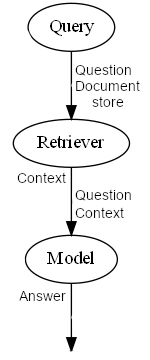
\includegraphics[width=0.35\linewidth]{fig/pipeline.png}
	\caption{\textbf{Pipeline diagram}, left are the outputs of thee node above, right are the inputs to the node below.}
	\label{fig:pipeline}
\end{figure}

The general outline of the pipeline can be observed in Figure \ref{fig:pipeline} and its components are briefly described in the following paragraphs.

\noindent We considered two approaches, the first one being the extractive approach.
In this approach, models try to find the answer in a given context, which is a task well suited for the data generated with the previously mentioned pipeline.
This approach has been shown to be reliable for simpler questions.
There are multiple limitations of this approach since models can accept only a limited length context and the answer might not always be contained in the context.
We implored two variants of BERT called DistilBERT~\cite{sanh2019distilbert} and RoBERTa~\cite{liu2019roberta} which have already been pre-trained on the SQuAD dataset.
% Our preliminary model was a smaller variant of BERT called DistilBERT~\cite{sanh2019distilbert} which has already been pre-trained on the SQuAD dataset.
% {\it Additional fine-tuning will have to be done after expanding the dataset. The full process will be explained here.}

\noindent Our second approach is generative.
Such models learn to generate a sequence of words from the input query (and context if provided).
The benefit of these models is that they should be able to answer more complex questions since they are not only extracting the answer from the context but generating the answer based on understanding the language and the provided context.
For this approach, we use the small and base version of the T5~\cite{T5} model which have been finetuned for question-answering on the SQuAD dataset.
% {\it This approach could be better suited for question-answer pairs that are written and not automatically generated, as we have no guarantee that the answer will be provided directly in the context, but may be paraphrased or expressed implicitly. The baseline models used for this approach will likely include T5 and LLaMA.}

\noindent Since both the extractive and generative approaches require contexts our pipeline has to provide one with the answer.
A sliding window passing through all possible contexts is feasible but would be computationally inefficient.
Therefore, we will employ a context retriever model which will identify a small number of relevant contexts to the given question.
We employ the DPR~\cite{karpukhin2020dense} model which was shown to outperform more traditional methods such as TF-IDF or BM25.
% {\it Here the DPR model will be used as the first part of the pipeline, to find and extract the required context, and its output will be fed to the QA model to return the answer.}
% \textbf{TODO: update}

\noindent To leverage the additional information contained in the provided data we fine-tune all of the components on the automatically generated data from the 2020 and 2022 reports, the combined data from the 2020 and 2022 (2042) reports, and the handwritten data.
We also test multiple combinations of the components since we can choose the extractive or generative model and the data that was used to finetune those models.

\subsection*{Evaluation}
For evaluation, we consider several metrics. Since SQuAD has its own evaluation benchmark, this is our first choice. 
The two main components of this benchmark are the percentage of exact matches between the predicted and the ground truth answers, and the average overlap (F1 score). 
The predictions and ground truths are transformed into bags of tokens, for which the overlap is calculated.
The second metric, BLEU~\cite{papineni2002bleu}, is a benchmark for evaluating translation models.
Its idea is to match the $n$-grams of the generated text, to those of the ground truth. These matches are then averaged geometrically.
Next, Bertscore~\cite{zhang2019bertscore}, leverages contextual embeddings to represent tokens, and then computes precision, recall, and F1 score using cosine similarity between the embeddings of the predicted answer and those of the ground truth.
% {\it Based on our dataset, we will also consider the SuperGLUE ReCoRD and MultiRC tasks in our evaluation.}
% \textbf{TODO: update}

%------------------------------------------------
\section*{Results}

\subsection*{Model performance}
\begin{table}[hbt]
	\caption{Extractive model results on test sets for different datasets. \textit{Fine} refers to the fine-tuned model, \textit{half} refers to fine-tuning on only half the train set.}
	\centering
    \label{tab:bert_fine_tuning}
    \scalebox{0.65}{
    	\begin{tabular}{c l || c c c | c | c c}
    		  & & \multicolumn{3}{c|}{Bertscore} & Bleu & \multicolumn{2}{c}{SQuAD}\\
    		& Model                & Precision & Recall & F1 & & Exact & F1 \\
            \hline \hline
            \multirow{6}{*}{\STAB{\rotatebox[origin=c]{90}{2020}}}
    		  & distil               & $90.59$ & $93.37$ & $91.91$ & $15.14$ & $44.64$ & $57.66$ \\
            & distil-fine-half     & $90.36$ & $93.13$ & $91.67$ & $15.74$ & $42.86$ & $55.33$ \\
            & distil-fine          & $90.48$ & $93.28$ & $91.81$ & $15.07$ & $42.86$ & $56.70$ \\
            \cmidrule(lr){2-8}
            & roberta              & $73.93$ & $91.90$ & $75.54$ & $39.55$ & $46.43$ & $57.20$ \\
            & roberta-fine-half    & $88.11$ & $93.82$ & $90.09$ & $32.04$ & $51.79$ & $63.45$ \\
            & roberta-fine         & $90.12$ & $94.08$ & $91.98$ & $39.53$ & $53.57$ & $65.24$ \\
            \hline \hline
            \multirow{6}{*}{\STAB{\rotatebox[origin=c]{90}{2022}}}
            & distil               & $86.95$ & $91.57$ & $88.44$ & $10.92$ & $31.78$ & $46.82$ \\
            & distil-fine-half     & $87.50$ & $91.86$ & $88.87$ & $14.78$ & $36.45$ & $48.95$ \\
            & distil-fine          & $86.91$ & $91.91$ & $88.24$ & $16.12$ & $37.38$ & $50.04$ \\
            \cmidrule(lr){2-8}
            & roberta              & $72.86$ & $91.10$ & $74.33$ & $25.21$ & $40.19$ & $53.39$ \\
            & roberta-fine-half    & $89.33$ & $93.43$ & $90.90$ & $39.22$ & $53.27$ & $66.67$ \\
            & roberta-fine         & $90.26$ & $93.36$ & $91.72$ & $37.61$ & $51.40$ & $66.48$ \\
            \hline \hline
            \multirow{6}{*}{\STAB{\rotatebox[origin=c]{90}{2042}}}
            & distil               & $85.94$ & $92.17$ & $87.49$ & $9.22$  & $37.32$ & $48.68$ \\
            & distil-fine-half     & $86.00$ & $92.33$ & $87.35$ & $10.97$ & $39.44$ & $50.65$ \\
            & distil-fine          & $88.13$ & $92.54$ & $89.52$ & $11.69$ & $38.73$ & $50.50$ \\
            \cmidrule(lr){2-8}
            & roberta              & $70.46$ & $91.12$ & $71.78$ & $26.46$ & $38.03$ & $46.47$ \\
            & roberta-fine-half    & $88.12$ & $93.60$ & $90.01$ & $28.95$ & $45.07$ & $57.82$ \\
            & roberta-fine         & $89.07$ & $93.64$ & $90.76$ & $32.09$ & $47.18$ & $59.32$ \\
            \hline \hline
            \multirow{4}{*}{\STAB{\rotatebox[origin=c]{90}{hand}}}
            & distil               & $87.71$ & $86.50$ & $87.04$ & $15.36$ & $15.79$ & $37.71$ \\
            & distil-fine          & $87.68$ & $88.28$ & $87.90$ & $37.81$ & $10.53$ & $45.52$ \\
            \cmidrule(lr){2-8}
            & roberta              & $56.82$ & $82.55$ & $57.13$ & $0.53$  & $5.26$  & $22.14$ \\
            & roberta-fine         & $75.83$ & $87.73$ & $79.33$ & $47.66$ & $15.79$ & $47.09$
            
    	\end{tabular}
     }
\end{table}

\begin{table}[hbt]
	\caption{Generative model results on test sets for different datasets. \textit{Fine} refers to the fine-tuned model, \textit{half} refers to fine-tuning on only half the train set.}
	\centering
    \label{tab:t5_fine_tuning}
    \scalebox{0.65}{
    	\begin{tabular}{c l || c c c | c }
    		  & & \multicolumn{3}{c|}{Bertscore} & Bleu \\
            & Model              & Precision & Recall & F1 & \\
            \hline \hline
            \multirow{6}{*}{\STAB{\rotatebox[origin=c]{90}{2020}}}
            & t5-small                & $96.87$ & $97.24$ & $97.04$ & $72.09$ \\
            & t5-small-finetuned-half & $97.34$ & $97.92$ & $97.62$ & $70.64$ \\
            & t5-small-finetuned      & $97.53$ & $98.15$ & $97.83$ & $70.65$ \\
            \cmidrule(lr){2-6}
            & t5-base                 & $87.88$ & $90.48$ & $89.12$ & $14.45$ \\
            & t5-base-finetuned-half  & $98.87$ & $99.19$ & $98.98$ & $82.33$ \\
            & t5-base-finetuned       & $98.75$ & $99.09$ & $98.91$ & $85.52$ \\
            \hline \hline
            \multirow{6}{*}{\STAB{\rotatebox[origin=c]{90}{2022}}}
            & t5-small                & $95.12$ & $95.10$ & $95.09$ & $64.80$ \\
            & t5-small-finetuned-half & $96.44$ & $96.62$ & $96.51$ & $69.52$ \\
            & t5-small-finetuned      & $97.22$ & $97.64$ & $97.41$ & $69.33$ \\
            \cmidrule(lr){2-6}
            & t5-base                 & $89.32$ & $91.81$ & $90.51$ & $13.38$ \\
            & t5-base-finetuned-half  & $98.57$ & $98.66$ & $98.61$ & $80.37$ \\
            & t5-base-finetuned       & $98.71$ & $98.78$ & $98.74$ & $81.92$ \\
            \hline \hline
            \multirow{6}{*}{\STAB{\rotatebox[origin=c]{90}{2042}}}
            & t5-small                & $95.07$ & $95.54$ & $95.28$ & $55.46$ \\
            & t5-small-finetuned-half & $96.89$ & $97.75$ & $97.30$ & $55.63$ \\
            & t5-small-finetuned      & $97.03$ & $98.16$ & $97.57$ & $54.31$ \\
            \cmidrule(lr){2-6}
            & t5-base                 & $88.29$ & $90.95$ & $89.55$ & $12.71$ \\
            & t5-base-finetuned-half  & $97.60$ & $98.16$ & $97.86$ & $61.03$ \\
            & t5-base-finetuned       & $98.07$ & $98.44$ & $98.25$ & $68.27$ \\
            \hline \hline
            \multirow{4}{*}{\STAB{\rotatebox[origin=c]{90}{hand}}}
            & t5-small                & $89.48$ & $86.39$ & $87.87$ & $6.74$ \\
            & t5-small-finetuned      & $92.26$ & $88.93$ & $90.52$ & $22.11$ \\
            \cmidrule(lr){2-6}
            & t5-base                 & $83.70$ & $84.70$ & $84.13$ & $12.81$ \\
            & t5-base-finetuned       & $93.21$ & $92.25$ & $92.68$ & $52.30$
            
    	\end{tabular}
     }
\end{table}

In Table~\ref{tab:bert_fine_tuning} and Table~\ref{tab:t5_fine_tuning} we can observe the results obtained by the extractive and generative models before and after additional fine-tuning.
We fine-tuned the models on the train splits of automatically generated data from 2020, 2022, and 2042, as well as on the handwritten data.

\noindent We observe that fine-tuning a model results in better metrics in most cases.
On the automatically generated data, we get good results without additional fine-tuning. We observe an increase of  1\% to 2\% after fine-tuning.
The biggest difference in performance is observed with the handwritten data, where the increase is much larger, depending on the model, especially for the BLEU score. Others perform very similarly before and after fine-tuning.
This could be expected since the automatically generated data resembled the data in SQuAD much more than the handwritten data.
Since all of the baseline models were already trained on SQuAD the information gained was much smaller when contrasted with fine-tuning on the handwritten data, which is more distinct. Thus the models were able to learn more information.

\noindent Using the automatically generated data we also tried fine-tuning the models on only half of the train set to see if training on less data impacts the models significantly.
We observed that most models performed worse, meaning that more data results in better metrics.
However, the metrics are not much higher so it is questionable if the additional work (filtering all of the automatically generated data) is worth the slight increase in performance.


%%%%%%%%%%%%%%%%%%
\subsection*{Performance of the pipeline}

\begin{table}[hbt]
	\caption{Pipeline results with fine-tuned models. }
	\centering
    \label{tab:pipeline}
    \scalebox{0.65}{
    	\begin{tabular}{c c l || c c c | c | c c}
    		  & & & \multicolumn{3}{c|}{Bertscore} & Bleu & \multicolumn{2}{c}{SQuAD}\\
    		& & Model                & Precision & Recall & F1 & & Exact match & F1 \\
            \hline \hline
            \multirow{8}{*}{\STAB{\rotatebox[origin=c]{90}{2042}}}
            & \multirow{4}{*}{\STAB{\rotatebox[origin=c]{90}{DPR}}}
            &  distil-fine   & $91.75$ & $91.41$ & $91.57$ & $12.22$ & $23.94$ & $27.64$ \\
            && roberta-fine  & $92.85$ & $92.84$ & $92.83$ & $29.09$ & $35.21$ & $37.89$ \\
            && t5-small-fine & $92.18$ & $92.50$ & $92.33$ & $15.24$ & / & / \\
            && t5-base-fine  & $91.64$ & $92.02$ & $91.81$ & $16.79$ & / & / \\
            \cmidrule(lr){2-9}
            & \multirow{4}{*}{\STAB{\rotatebox[origin=c]{90}{DPR-fine}}}
    		  &  distil-fine   & $91.88$ & $91.61$ & $91.73$ & $15.18$ & $27.46$ & $31.70$ \\
            && roberta-fine  & $93.18$ & $93.03$ & $93.09$ & $33.23$ & $36.62$ & $39.93$ \\
            && t5-small-fine  & $91.94$ & $92.68$ & $92.04$ & $14.53$ & / & / \\
            && t5-base-fine & $92.06$ & $92.49$ & $92.25$ & $18.28$ & / & / \\
            \hline \hline
            \multirow{8}{*}{\STAB{\rotatebox[origin=c]{90}{hand}}}
            & \multirow{4}{*}{\STAB{\rotatebox[origin=c]{90}{DPR}}}
            &  distil-fine   & $86.98$ & $86.94$ & $86.93$ & $0.0$   & $4.76$ & $11.58$ \\
            && roberta-fine  & $88.15$ & $87.33$ & $87.63$ & $4.61$  & $4.76$ & $21.53$ \\
            && t5-small-fine & $88.78$ & $87.44$ & $88.04$ & $13.48$ & / & / \\
            && t5-base-fine  & $86.11$ & $88.20$ & $87.06$ & $24.60$ & / & / \\
            \cmidrule(lr){2-9}
            & \multirow{4}{*}{\STAB{\rotatebox[origin=c]{90}{DPR-fine}}}
    		  &  distil-fine   & $87.41$ & $87.19$ & $87.25$ & $0.0$ & $4.76$ & $16.87$ \\
            && roberta-fine  & $88.78$ & $87.75$ & $88.21$ & $5.10$ & $14.29$ & $27.57$ \\
            && t5-small-fine & $86.92$ & $85.23$ & $86.03$ & $0.88$ & / & / \\
            && t5-base-fine  & $85.45$ & $87.42$ & $86.38$ & $18.75$ & / & / \\
        
    	\end{tabular}
     }
\end{table}

In Table~\ref{tab:pipeline} we can observe the results obtained using fine-tuned models in combination with a DPR that has or hasn't been fine-tuned (on automatically generated data).
The DPR retrieves the contexts from both of the reports in the case of 2042 data and only from the 2022 report for the handwritten data. 
We can see that fine-tuning the DPR has a positive effect in most cases as a higher number of exact matches are achieved (alongside an increase in other metrics).
This means that the DPR managed to retrieve more relevant contexts meaning that the models can provide better answers.
% The exception to this are the generative models fine-tuned on handwritten data using a fine-tuned DPR.

\subsection*{Qualitative analysis}

\begin{table}[hbt]
	\caption{Qualitative analysis of the entire pipeline on 2042 data and handwritten data}
	\centering
    \label{tab:pipeline_qualitative}
    \scalebox{0.75}{
    	\begin{tabular}{c l || c c c c | c c c c | c}
    		  &       & \multicolumn{4}{c|}{Correctness} & \multicolumn{4}{c|}{Sensibility} & No answer \\
            & Model & 1 & 2 & 3 & avg & 1 & 2 & 3 & avg & \\
            \hline \hline
            \multirow{4}{*}{\STAB{\rotatebox[origin=c]{90}{2042}}}
            & distilbert    & 13 & 1 & 7 & 1.71 & 7 & 5 & 9 & 2.10 & 0 \\
            & roberta       & 13 & 1 & 7 & 1.71 & 7 & 5 & 9 & 2.10 & 0 \\
            & t5 small      & 13 & 1 & 7 & 1.71 & 7 & 6 & 8 & 2.05 & 0 \\
            & t5 base       & 13 & 1 & 7 & 1.71 & 7 & 5 & 9 & 2.10 & 0 \\
            \hline
            \multirow{4}{*}{\STAB{\rotatebox[origin=c]{90}{hand}}}
            & distilbert    & 17 & 3 & 1 & 1.24 & 8 & 6 & 7 & 1.95 & 0 \\
            & roberta       & 18 & 3 & 0 & 1.14 & 11 & 4 & 6 & 1.76 & 0 \\
            & t5 small      & 16 & 5 & 0 & 1.24 & 12 & 3 & 6 & 1.71 & 7 \\
            & t5 base       & 17 & 3 & 1 & 1.24 & 14 & 1 & 6 & 1.62 & 0 \\
    	\end{tabular}
     }
\end{table}

\begin{table*}[hbt]
	\caption{Examples of retrieved contexts and obtained answers with the pipeline. An answer generated with ChatGPT is provided for comparison.}
 %In the first example the retreived context is ''correct`` and all the models answer correctly. In the second the retrieved context is relevant but not the one expected so we get a meaningful answer but different than the ground truth one. In the last example the retrieved context only mentions one thing in the question and does not contain any relevant information.}
	\centering
	\label{tab:examples}
    \scalebox{0.9}{
	\begin{tabular}{l}
        \hline \hline
        % 2042: 12
        \textbf{Question}: How many Slovenian companies joined the GREENVISION initiative? \textbf{GT Answer}: almost 100\\
        \textbf{Retreived context}: NLB Group in numbers (as at 31 December 2022)\\
        • An extensive network of 440 branches in all markets where NLB Group operates.\\
        • More than 2.7 million active customers.\\
        • With successful operations, NLB Group generated a record high profit of €446.9 million in 2022, with the acquisition \\ of N Banka in March significantly influencing the full-year business results of the Group.\\
        • The balance sheet total of the NLB Group amounts to €24.2 billion.\\
        \hline
		\textbf{Answers} $\mid$ distilbert: ''440'' $\mid$ roberta: ''440'' $\mid$ t5-small: ''440'' $\mid$ t5-base: ''440''\\
        \hline
        \textbf{ChatGPT Answer}: Based on the provided context, the number of branches NLB Group has in all markets where it operates is 440. \\
        \hline \hline
        % 2042: 5
        \textbf{Question}: How much did the bank reduce the use of paper in 2022 compared to the previous year? \textbf{GT Answer}: 19\%\\
        \textbf{Retreived context}: In 2022, another step to achieving this goal has been made as paper usage (prints) was reduced \\
        by 17\% compared to 2021. Thus, we saved 866 trees. Paper usage in NLB was lower by 26\%, which is the highest\\
        reduction group – wide. All banking subsidiaries experienced reduction as well, ranging from 8\% to 19\%, respectively.\\
        \hline
		\textbf{Answers} $\mid$ distilbert: ''17\%'' $\mid$ roberta: ''17\%'' $\mid$ t5-small: ''17\%'' $\mid$ t5-base: ''17\%''\\
        \hline
        \textbf{ChatGPT Answer}: Based on the given context, the bank reduced the use of paper by 17\% compared to the previous year\\
        (2021). However, the exact amount of paper usage in 2021 or any specific quantity of paper used is not mentioned.\\
        \hline \hline
        % handwritten 13
        \textbf{Question}: How much new green loan NLB Group generated for retail clients? \textbf{GT Answer}: Over €53 million\\
        \textbf{Retreived context}: NLB Green Housing loan (SDG 11,12,13) Purposes: for purchasing or building a passive house, for\\
        purchase and installation of solar power plants with or w/o battery, for heat pumps, charging stations, IR panels, and gas\\
        boilers 2. NLB Green partner loan (SDG 11, 12,13) Purposes: for purchase and installation of solar power plants with or\\
        w/o battery, for heat pumps, charging stations, IR panels, and gas boilers NLB Group finances corporate clients for\\
        projects such as: • wind farms, • solar power plants, • energy-efficient buildings. ››› 1. For more information\\
        about client engagement, please refer to: Sustainability Report 2022 p. 12 ››› 2. \\
        \hline
		\textbf{Answers} $\mid$ distilbert: ''13'' $\mid$ roberta: ''›››'' $\mid$ t5-small: ''None'' $\mid$ t5-base: ''NLB Green partner loan (SDG 11, 12,13)''\\
        \hline
        \textbf{ChatGPT Answer}: The context provided does not mention the specific amount of new green loans generated by NLB Group\\
        for retail clients. It only outlines the types of green loans offered by NLB Group, such as the NLB Green Housing loan and NLB\\
        Green partner loan, along with their purposes.\\
        \hline \hline
        
	\end{tabular}
    }
\end{table*}

\noindent To better gauge how well the entire pipeline works we look through the entire test set (21 examples) of handwritten questions and a subset of the automatically generated questions (21 examples that were selected arbitrarily).
We score the answers based on sensibility - how sensible the retrieved context and thus the extracted/generated answer and correctness - how close to the expected answer is to the obtained one.
We assign a number from 1 (worst) to 3 (best) for each of the examples and marked the number of questions for which we get no answer - the model thinks it can't answer the question from the provided context.

\noindent We can observe these results in Table \ref{tab:pipeline_qualitative}.
The results are quite poor since a lot of the time the ''wrong'' context is retrieved.
We can observe that sensibility always scores better than correctness since the context usually contains some information that is related to the question - the answer could be considered correct but is not the same as the ground truth.
We see that the simpler questions from the automatically generated data yield better results than the handwritten ones.
This is not surprising as some of the handwritten questions are fairly long and complex.
From the model and pipeline evaluation, we would expect that the generative models perform slightly better than the extractive ones at least in the case of more complex (handwritten) data.
The scores do not indicate this without looking at the number of times that we get the answer ''None''.
The small variant of T5 correctly identifies that the retrieved context does not contain the answer 7 times. Since it's the only one that does this we would pick it as the best model.
% TODO: base model doesn't do this -should we write this?

\noindent In Table \ref{tab:examples} we can see 3 examples of retrieved contexts and the obtained answers from each model.
We can see that when the context contains the ground truth answer we obtain the correct answer (1st example), when the context is relevant we get a sensible answer which may not be exactly the one we defined as the ground truth (2nd example) and when the context is incorrect we get incorrect answers or the answer ''None'' indicating that the model could not find the answer in the provided context.
For comparison, we also include the answers obtained from a significantly larger model (ChatGPT). As expected the use of a larger model yields much better results.

%Use the results section to present the final results of your work. Present the results in a objective and scientific fashion. Use visualisations to convey your results in a clear and efficient manner. When comparing results between various techniques use appropriate statistical methodology.

%\subsection*{More random text}

%This text is inserted only to make this template look more like a proper report. Lorem ipsum dolor sit amet, consectetur adipiscing elit. Etiam blandit dictum facilisis. Lorem ipsum dolor sit amet, consectetur adipiscing elit. Interdum et malesuada fames ac ante ipsum primis in faucibus. Etiam convallis tellus velit, quis ornare ipsum aliquam id. Maecenas tempus mauris sit amet libero elementum eleifend. Nulla nunc orci, consectetur non consequat ac, consequat non nisl. Aenean vitae dui nec ex fringilla malesuada. Proin elit libero, faucibus eget neque quis, condimentum laoreet urna. Etiam at nunc quis felis pulvinar dignissim. Phasellus turpis turpis, vestibulum eget imperdiet in, molestie eget neque. Curabitur quis ante sed nunc varius dictum non quis nisl. Donec nec lobortis velit. Ut cursus, libero efficitur dictum imperdiet, odio mi fermentum dui, id vulputate metus velit sit amet risus. Nulla vel volutpat elit. Mauris ex erat, pulvinar ac accumsan sit amet, ultrices sit amet turpis.

%Phasellus in ligula nunc. Vivamus sem lorem, malesuada sed pretium quis, varius convallis lectus. Quisque in risus nec lectus lobortis gravida non a sem. Quisque et vestibulum sem, vel mollis dolor. Nullam ante ex, scelerisque ac efficitur vel, rhoncus quis lectus. Pellentesque scelerisque efficitur purus in faucibus. Maecenas vestibulum vulputate nisl sed vestibulum. Nullam varius turpis in hendrerit posuere.

%Nulla rhoncus tortor eget ipsum commodo lacinia sit amet eu urna. Cras maximus leo mauris, ac congue eros sollicitudin ac. Integer vel erat varius, scelerisque orci eu, tristique purus. Proin id leo quis ante pharetra suscipit et non magna. Morbi in volutpat erat. Vivamus sit amet libero eu lacus pulvinar pharetra sed at felis. Vivamus non nibh a orci viverra rhoncus sit amet ullamcorper sem. Ut nec tempor dui. Aliquam convallis vitae nisi ac volutpat. Nam accumsan, erat eget faucibus commodo, ligula dui cursus nisi, at laoreet odio augue id eros. Curabitur quis tellus eget nunc ornare auctor.


%------------------------------------------------

\section*{Discussion}
% Thus far, we have identified the main approaches for solving our problem and defined the pipeline.
% We started by fine tuning a model for the extractive approach and shown that fine tuning on our domain specific data improves the performance of the model.
% When we receive the data written by the banking experts we plan on using that data to fine tune our models as it should be of better quality.
% Knowing that this approach works we plan on adapting a context retriever to extract the relevant contexts from the annual reports.
% After this, we plan to fine tune additional model(s) for the extractive approach and test the generative approach.
% Finally, we plan to identifying more realistic evaluation protocols including human evaluation where we would manually check a sample of the answers generated by the models.

\noindent There are two important factors to consider when drawing conclusions from the obtained results. These factors are the data and the models as well as the pipeline as a whole. We believe that each of these two factors played an important role in the end results and making alterations to each of them could improve the results.

\noindent First let's consider the data. We were somewhat limited by the data that was available to us. It hasn't been mentioned thus far but we generated over 4000 question-context-answer pairs, that were then filtered by the NLB banking professionals, to only include those that would be useful to them. The remaining 500 pairs, together with the handwritten examples, provide a good starting point to fine-tune the models. However, better results could be achieved with more data. This especially seems to be the case with the DPR model, since the pipeline is to some extent bottle-necked by its first component, which was noticeable during the qualitative analysis. Better results could also be achieved by using more higher-quality data. As stated previously the improvements seen when fine-tuning using the handwritten data are the greatest, which is the desired result. Having more data of this type could increase the performance beyond the results reported here. This wouldn't just allow us to answer more complex questions, but also achieve better results with smaller models. We could also expect better results, if we only focused on one type of questions, for example, one of the ones mentioned at the end of Section~\ref{sec:datasets}.

\noindent Qualitative analysis of the pipeline provided valuable insights into its functionality. The main takeaway was that in order to achieve better performance of the whole pipeline, we would need to improve the DPR. This could be done in a couple of ways, one being the already mentioned fine-tuning with more data. Another possible method would involve modifying the retriever node such that it returns more than one context in the hopes of obtaining one that actually has the answer. The pipeline could also be improved by improving the second part, that being the model itself. One of the limitations that the models we used had, was the length of accepted contexts. Implementing some Long Form Question-Answering (LFQA)~\cite{faneli5} models could possibly yield better results, as these can not only accept longer questions but process much bigger contexts as well, than the models we used. Another obvious improvement would be to use larger models. As we noticed, ChatGPT performed much better than our fine-tunned models, thus we can only expect that using it, LLaMA, LaMDA~\cite{thoppilan2022lamda} or BART~\cite{lewis2019bart} as part of the pipeline would yield better results. This would, however, require much more computational power than was available to us.

\noindent Lastly let's consider the comparison between extractive and generative models. During our testing, we saw much better results when using the ladder. Extractive models have a downside, in that they are looking for a substring in the context that would answer the question. Generative models don't have that limitation, and in fact, every larger model listed in the previous paragraph is a generative model. While extractive models are easier to train, they don't offer a significantly better cost-to-performance ratio, for us to consider them in the final product.


%Use the Discussion section to objectively evaluate your work, do not just put praise on everything you did, be critical and exposes flaws and weaknesses of your solution. You can also explain what you would do differently if you would be able to start again and what upgrades could be done on the project in the future.


%------------------------------------------------

\section*{Acknowledgments}
Firstly we would like to thank our faculty advisor prof. dr. Marko Robnik Šikonja for providing irreplaceable guidance and advice. We would also like to thank our client dr. Branislava Sandrih Todorović and the NLB group at large for their cooperation. And lastly our industry advisor Grega Jerkić for helping set the correct path and the foundations for us to build upon.

%Here you can thank other persons (advisors, colleagues ...) that contributed to the successful completion of your project.


% \cleardoublepage
\clearpage
%----------------------------------------------------------------------------------------
%	REFERENCE LIST
%----------------------------------------------------------------------------------------
\bibliographystyle{unsrt}
\bibliography{report}

\end{document}